\documentclass[]{article}
\usepackage{preambule}
\usepackage{subcaption}
\usepackage[accepted]{icml2016}

\title{DANN with some toy datasets}
\author{Victor}
\date{}

\begin{document}
\maketitle

{
\hypersetup{linkcolor=black}
\setcounter{tocdepth}{3}
\tableofcontents
}
\section{Moon dataset}\label{moon-dataset}

L'exemple des 2 lunes imbriquées est un problème non linéaire simple. Un
réseaux de neurone à 1 couche caché de 3 neurones permet de le résoudre.

\begin{figure}[htbp]
\centering
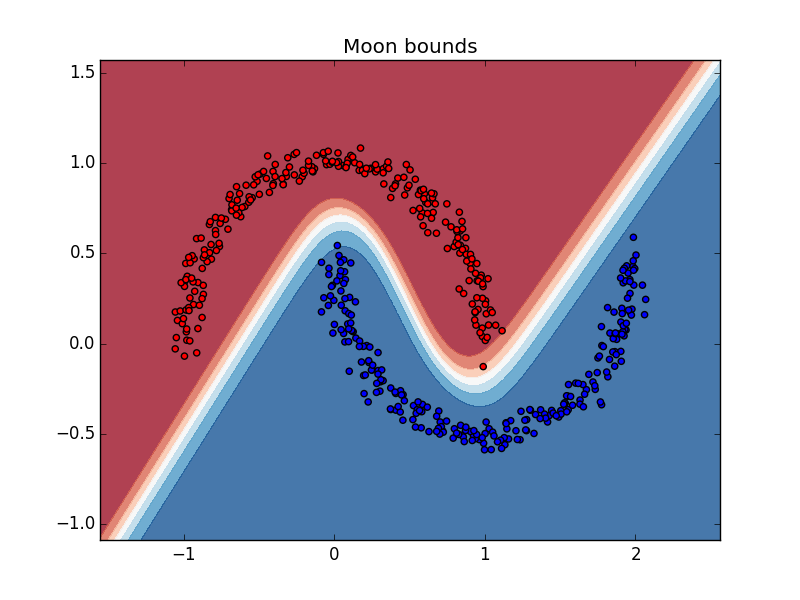
\includegraphics[width=.5\textwidth]{fig/moon-bound-0.png}
\caption{Moon classique}
\end{figure}


On peut simuler un problème d'adaptation en applicant une petite
transformation sur ces données.

\subsection{Rotation}\label{rotation}

Avec une rotation de 35 degrés le réseau de base perd une partie de ses
performances.

\begin{figure*}[htbp]
\centering
\begin{subfigure}[htbp]{.45\textwidth}
\centering
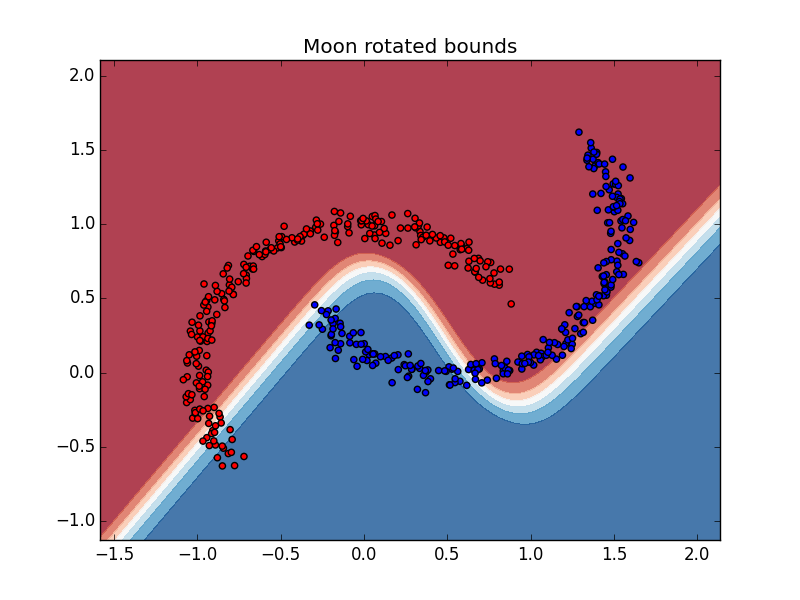
\includegraphics{fig/moon-rot-bound-0.png}
\caption{Moon après une rotation de 35 degrés. Les performances ont
diminuées.}
\end{subfigure}
\begin{subfigure}[htbp]{.45\textwidth}
\centering
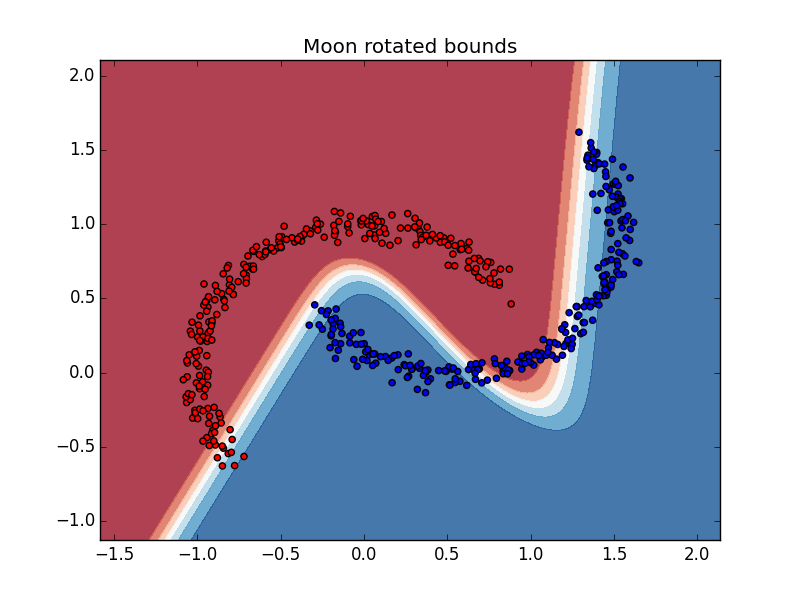
\includegraphics{fig/moon-rot-bound-1.png}
\caption{Moon après une rotation de 35 degrés. En utilisant un DANN.}
\end{subfigure}
\end{figure*}


\begin{figure*}[htbp]
\centering
\begin{subfigure}[htbp]{.45\textwidth}
\centering
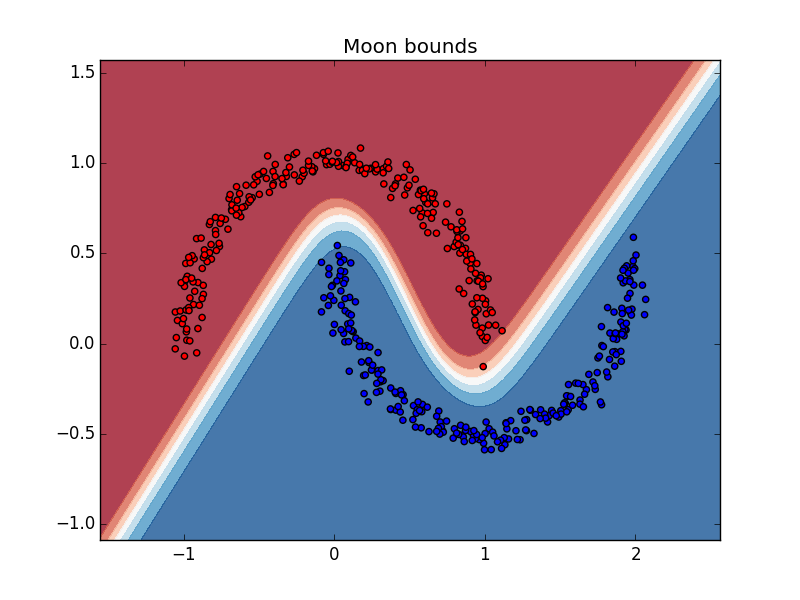
\includegraphics{fig/moon-bound-0.png}
\caption{Moon (donnée originale). Avant l'utilisation du DANN.}
\end{subfigure}
\begin{subfigure}[htbp]{.45\textwidth}
\centering
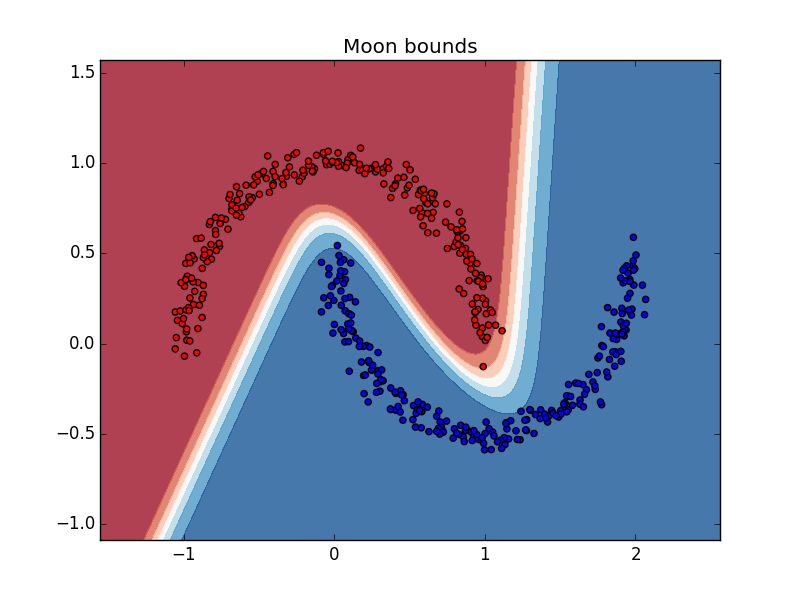
\includegraphics{fig/moon-bound-1.png}
\caption{Moon (donnée originale). Le DANN ne fait pas perdre de
performances sur ce datasaet.}
\end{subfigure}
\caption{En applicant un DANN on peut partiellement corriger ce problème
($\lambda_D=0.7$)}
\end{figure*}

\subsection{Matrice à dominance
diagonale}\label{matrice-uxe0-dominance-diagonale}

Une autre transformation consiste à appliquer une matrice à dominance
diagonale aux données:

\[ x \gets A.x \] où $A$ est une matrice $(2\times2)$ générée
aléatoirement.

\begin{figure*}[htbp]
\centering
\begin{subfigure}[htbp]{.45\textwidth}
\centering
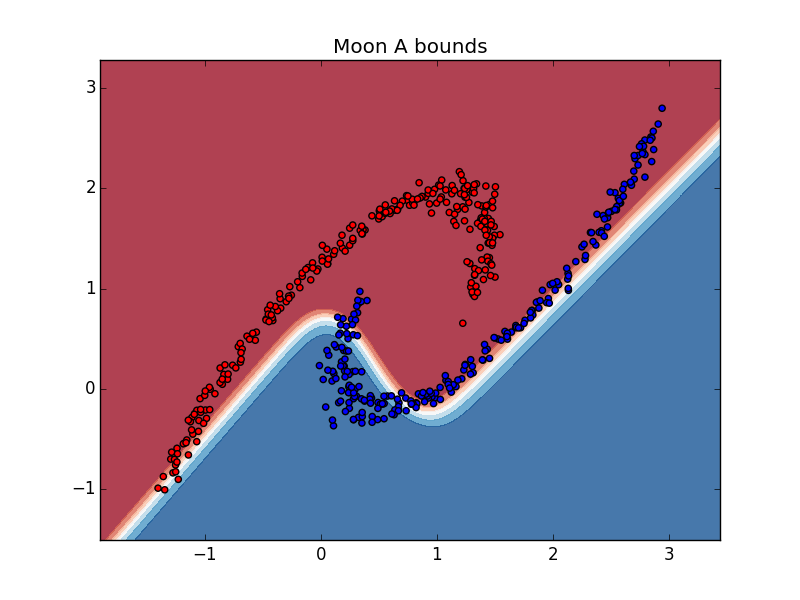
\includegraphics{fig/moon-A-bound-0.png}
\caption{Moon après transformation. Sans utilisation du DANN}
\end{subfigure}
\begin{subfigure}[htbp]{.45\textwidth}
\centering
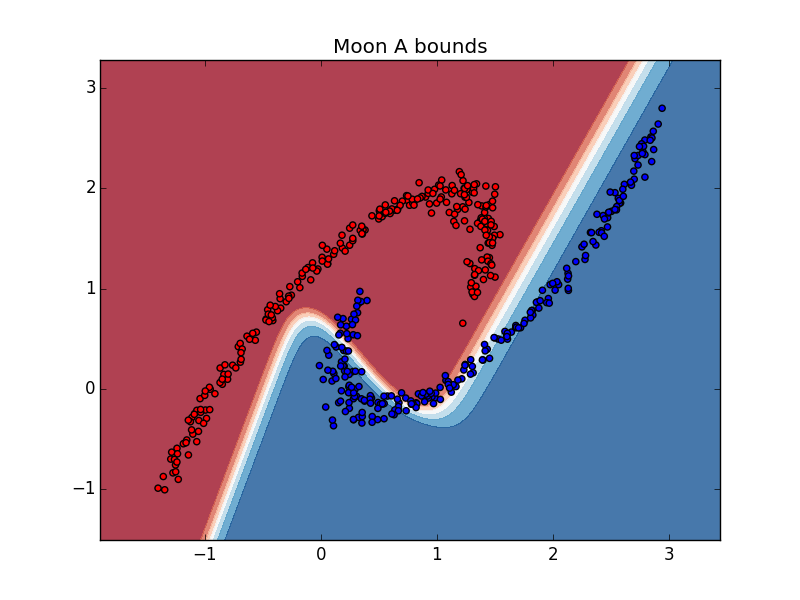
\includegraphics{fig/moon-A-bound-1.png}
\caption{Moon après transformation. En utilisant le DANN}
\end{subfigure}
\end{figure*}

\end{document}
